%
% Electronic Homework Template
% Modified from Jeremy Buhler's WUSTL CSE Template

\documentclass[11pt]{article}
\usepackage[left=0.7in,right=0.7in,top=0.7in,bottom=0.7in,headheight=14pt]{geometry}
\usepackage{helvet}
\usepackage{fancyhdr} % for header
\usepackage{caption}
\usepackage{subcaption}
\usepackage{float}
\usepackage{graphicx} % for figures
\usepackage{amsmath}  % for extended math markup
\usepackage{amssymb}
\usepackage[bookmarks=false]{hyperref} % for URL embedding
\renewcommand{\baselinestretch}{1.1}

%%%%%%%%%%%%%%%%%%%%%%%%%%%%%%%%%%%%%%%%%%%%%%%%%%%%%%%%%%%%%%%%%%%%%%%%

% create header and footer for every page
\pagestyle{fancy}
\fancyhf{}
\cfoot{\thepage}

%%%%%%%%%%%%%%%%%%%%%%%%%%%%%%%%%%%%%%%%%%%%%%%%%%%%%%%%%%%%%%%%%%%%%%

% Bibliography setup
\usepackage[authoryear]{natbib}
\bibliographystyle{chicago} % Cite Chicago style with \citep

%%%%%%%%%%%%%%%%%%%%%%%%%%%%%%%%%%%%%%%%%%%%%%%%%%%%%%%%%%%%%%%%%%%%%%

\begin{document}

\section*{Results}
We used \texttt{pyunlocbox} as the implementation for the FISTA algorithm. To select the optimal amount of regularization, we tried $\lambda$ values ranging from $10$ to $10^{-5}$ and created an L-curve. In all three cases (i.e. 540, 270, and 90 views), we found that $\lambda = 10^{-3}$ gave the optimal reconstruction (Figure~\ref{fig:lcurves}). The reconstruction from the full sinogram for all values of $\lambda$ is shown in Supplemental Figure~\ref{fig:fullReconstructions}.

% L-curves
\begin{figure}[h]
	\begin{subfigure}[t]{0.3\textwidth}
		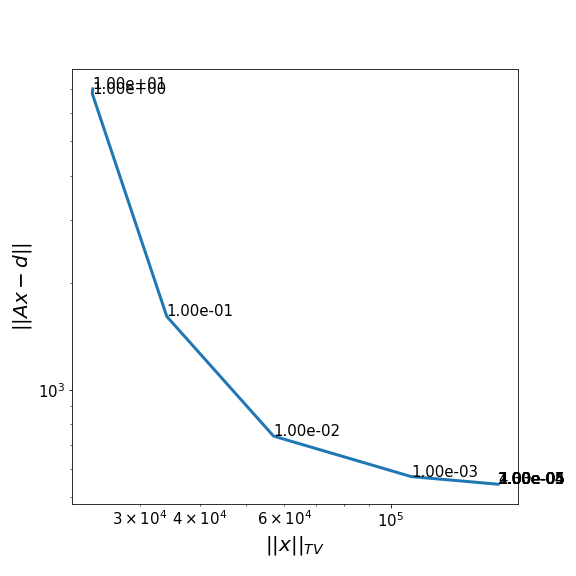
\includegraphics[width=\linewidth]{results/fistaFullLcurve.png}
		\caption{Full sinogram}
		\label{fig:lcurvefull}
	\end{subfigure}
	\hfill
	\begin{subfigure}[t]{0.3\textwidth}
		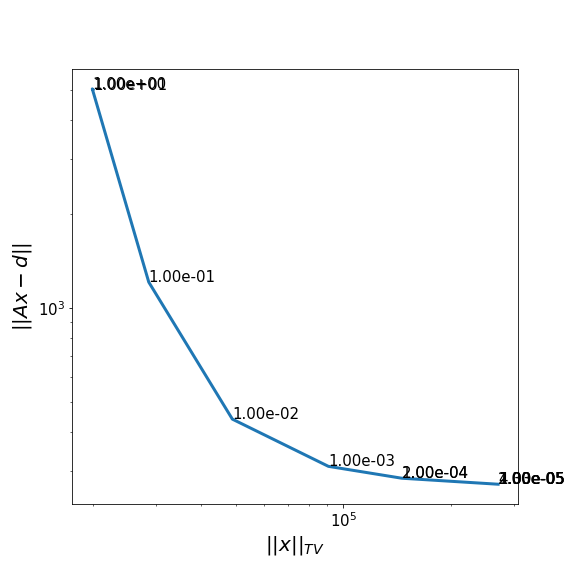
\includegraphics[width=\linewidth]{results/fista270Lcurve.png}
		\caption{270 views}
		\label{fig:lcurve270}
	\end{subfigure}
	\hfill
	\begin{subfigure}[t]{0.3\textwidth}
		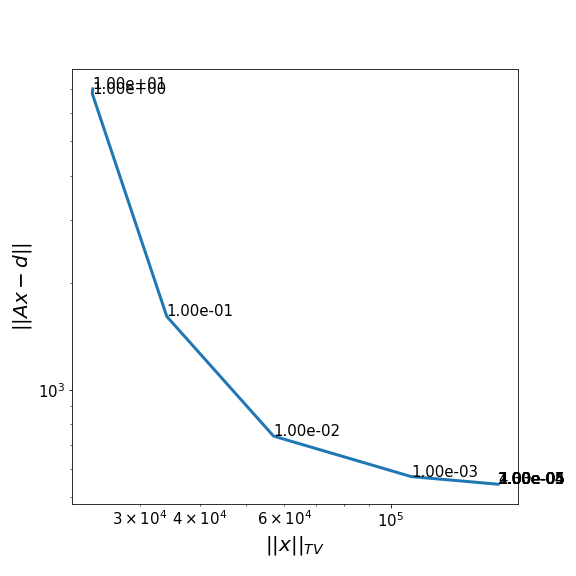
\includegraphics[width=\linewidth]{results/fistaFullLcurve.png}
		\caption{90 views}
		\label{fig:lcurve90}
	\end{subfigure}
	
	\caption{L-curves for FISTA reconstruction of image.}
	\label{fig:lcurves}
\end{figure}

We compared the image reconstructed with FISTA to reconstructions with SART. We chose to implement SART as our stationary method because it is less prone to overfitting than ART and converges faster than SIRT. We assessed image quality using two metrics, the structural similarity (SSIM) index and the mean squared error (MSE). We computed these metrics on the full image and on a defined region of interest (ROI). We set our ROI to cover pixel rows 175-220 and pixel columns 100-140 because the image has complex shapes in this region. The reconstructed images for 540, 270, and 90 views are shown in Figures~\ref{fig:comparisonfull},~\ref{fig:comparison270}, and~\ref{fig:comparison90}, respectively. The SSIM metrics are shown in Table~\ref{tab:ssim} and the MSE metrics are shown in Tabls~\ref{tab:mse}. In virtually every case, FISTA outperforms SART. However, the reconstruction from 90 views over the ROI is better with SART than with FISTA.

% SSIM metrics
\begin{table}[h]
	\centering
	\begin{tabular}{|c|c|c|c|c|}
		\hline
		\textbf{Number of views} & \textbf{FISTA} & \textbf{FISTA ROI} & \textbf{SART} & \textbf{SART ROI} \\
		\hline
		540 & 0.874 & 0.924 & 0.885 & 0.855 \\
		270 & 0.880 & 0.872 & 0.877 & 0.849 \\
		90  & 0.872 & 0.706 & 0.792 & 0.741 \\
		\hline
	\end{tabular}
	\caption{SSIM of image reconstructions.}
	\label{tab:ssim}
\end{table}

% MSE metrics
\begin{table}[h]
	\centering
	\begin{tabular}{|c|c|c|c|c|}
		\hline
		\textbf{Number of views} & \textbf{FISTA} & \textbf{FISTA ROI} & \textbf{SART} & \textbf{SART ROI} \\
		\hline
		540 & 35.24 & 115.76 & 40.91 & 244.75 \\
		270 & 39.18 & 207.21 & 43.62 & 251.27 \\
		90  & 62.37 & 471.45 & 80.66 & 397.23 \\
		\hline
	\end{tabular}
	\caption{MSE of image reconstructions.}
	\label{tab:mse}
\end{table}

% FISTA and SART side by side: full sinogram
\begin{figure}[H]
	\centering
	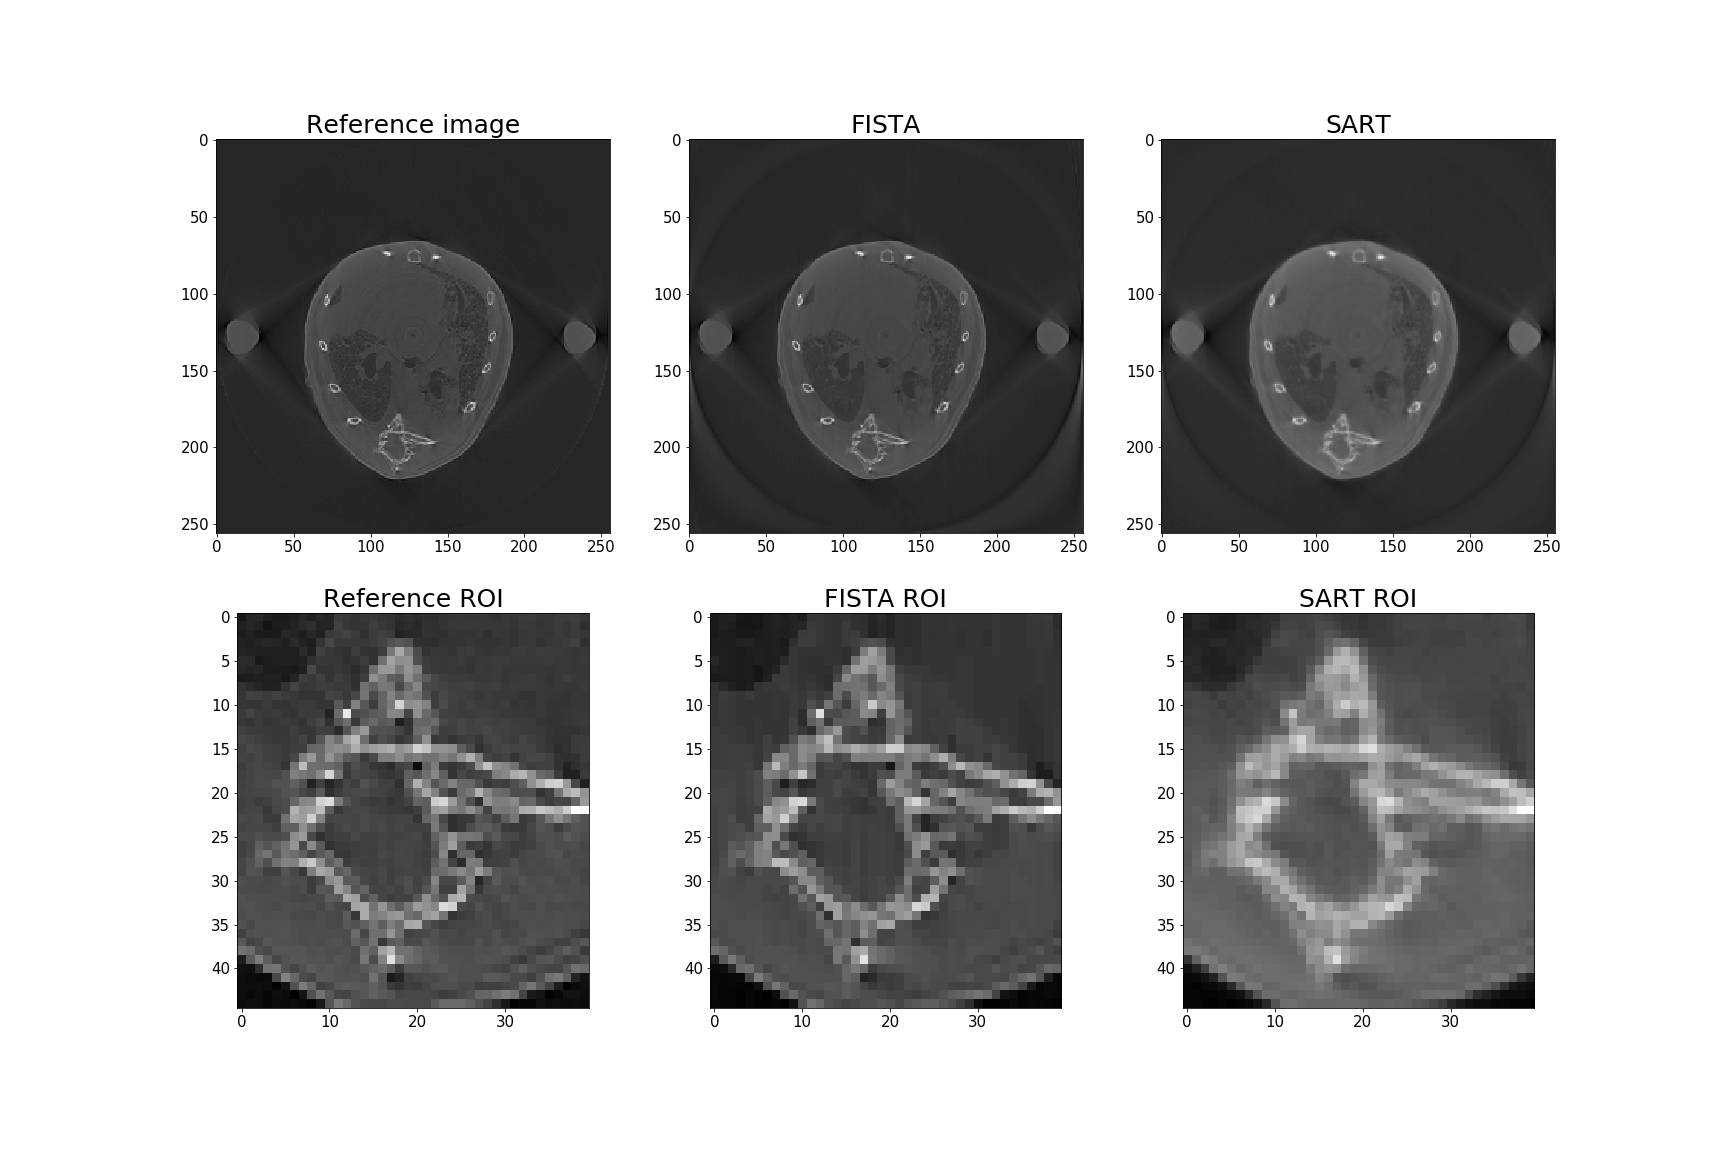
\includegraphics[height=0.35\paperheight]{results/comparisonFull.png}
	\caption{Reconstructed image using FISTA and SART from the full sinogram.}
	\label{fig:comparisonfull}
\end{figure}

% FISTA and SART side by side: 270
\begin{figure}[H]
	\centering
	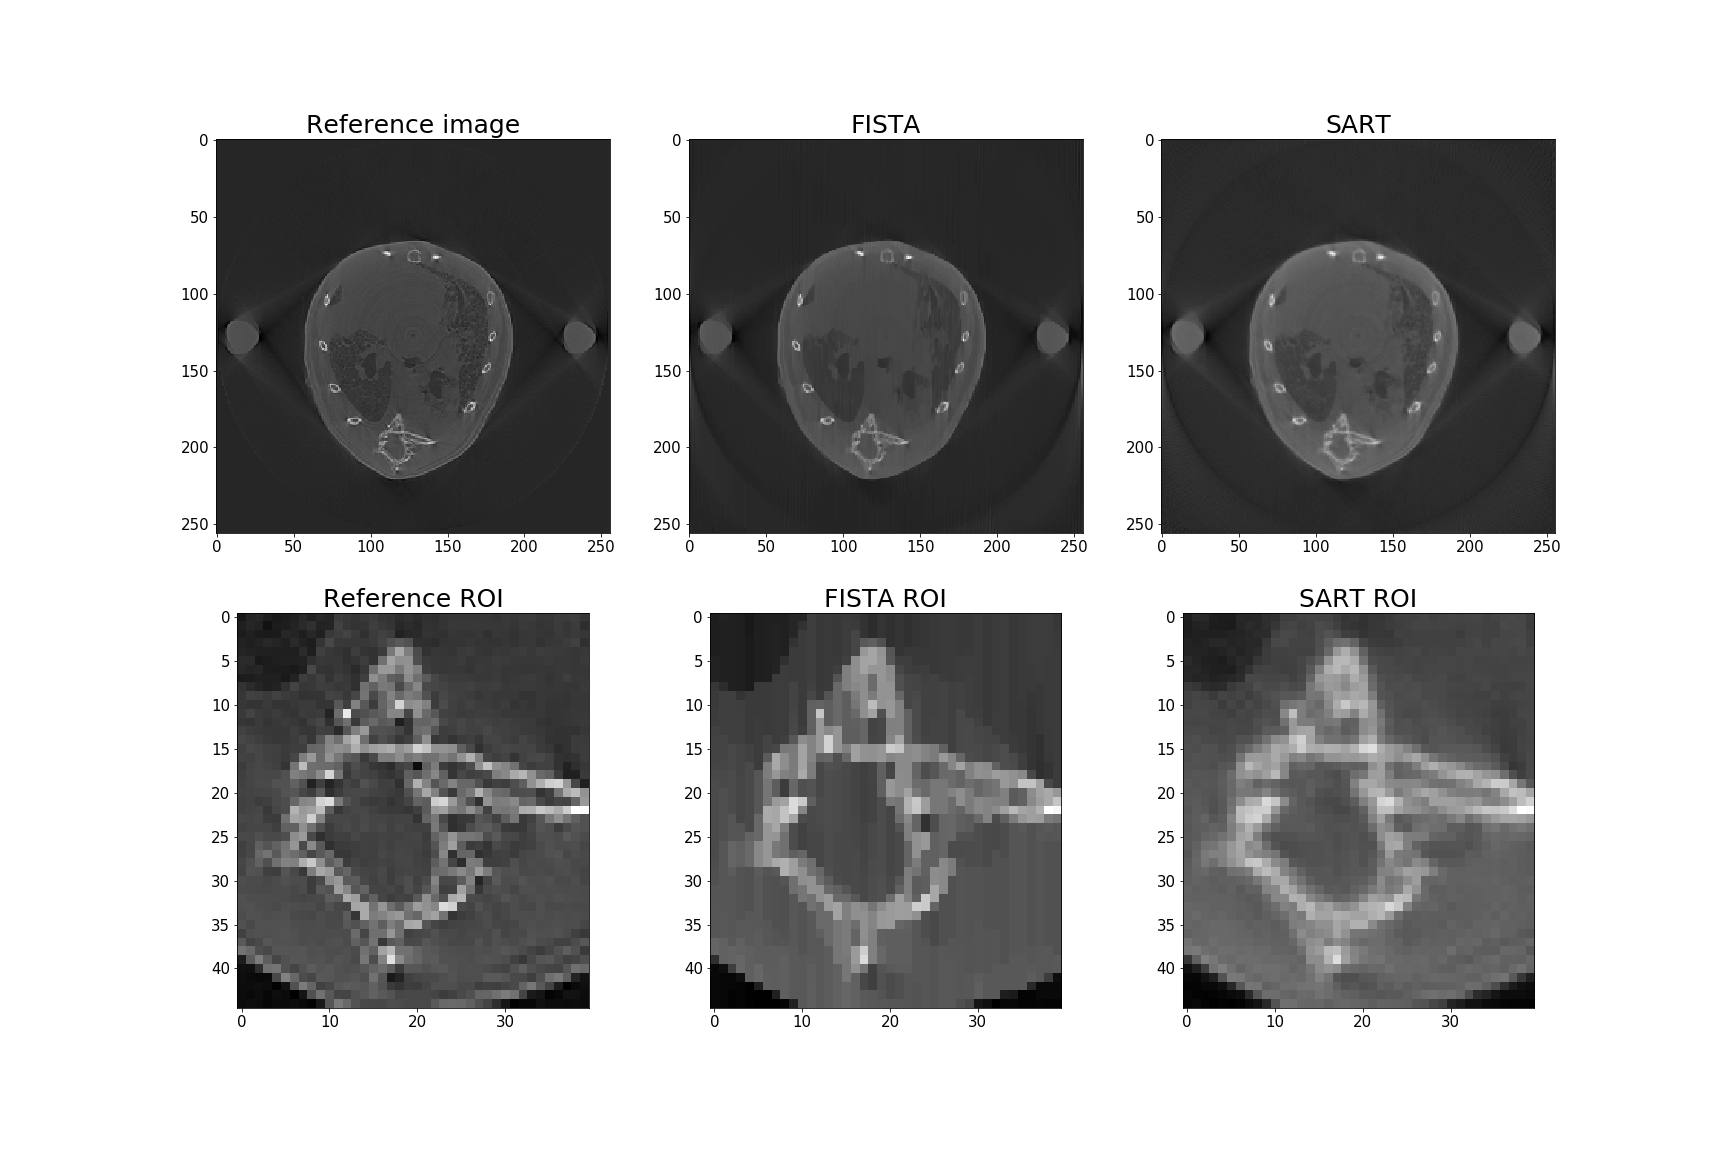
\includegraphics[height=0.35\paperheight]{results/comparison270.png}
	\caption{Reconstructed image using FISTA and SART from the 270 views.}
	\label{fig:comparison270}
\end{figure}

% FISTA and SART side by side: 90
\begin{figure}[H]
	\centering
	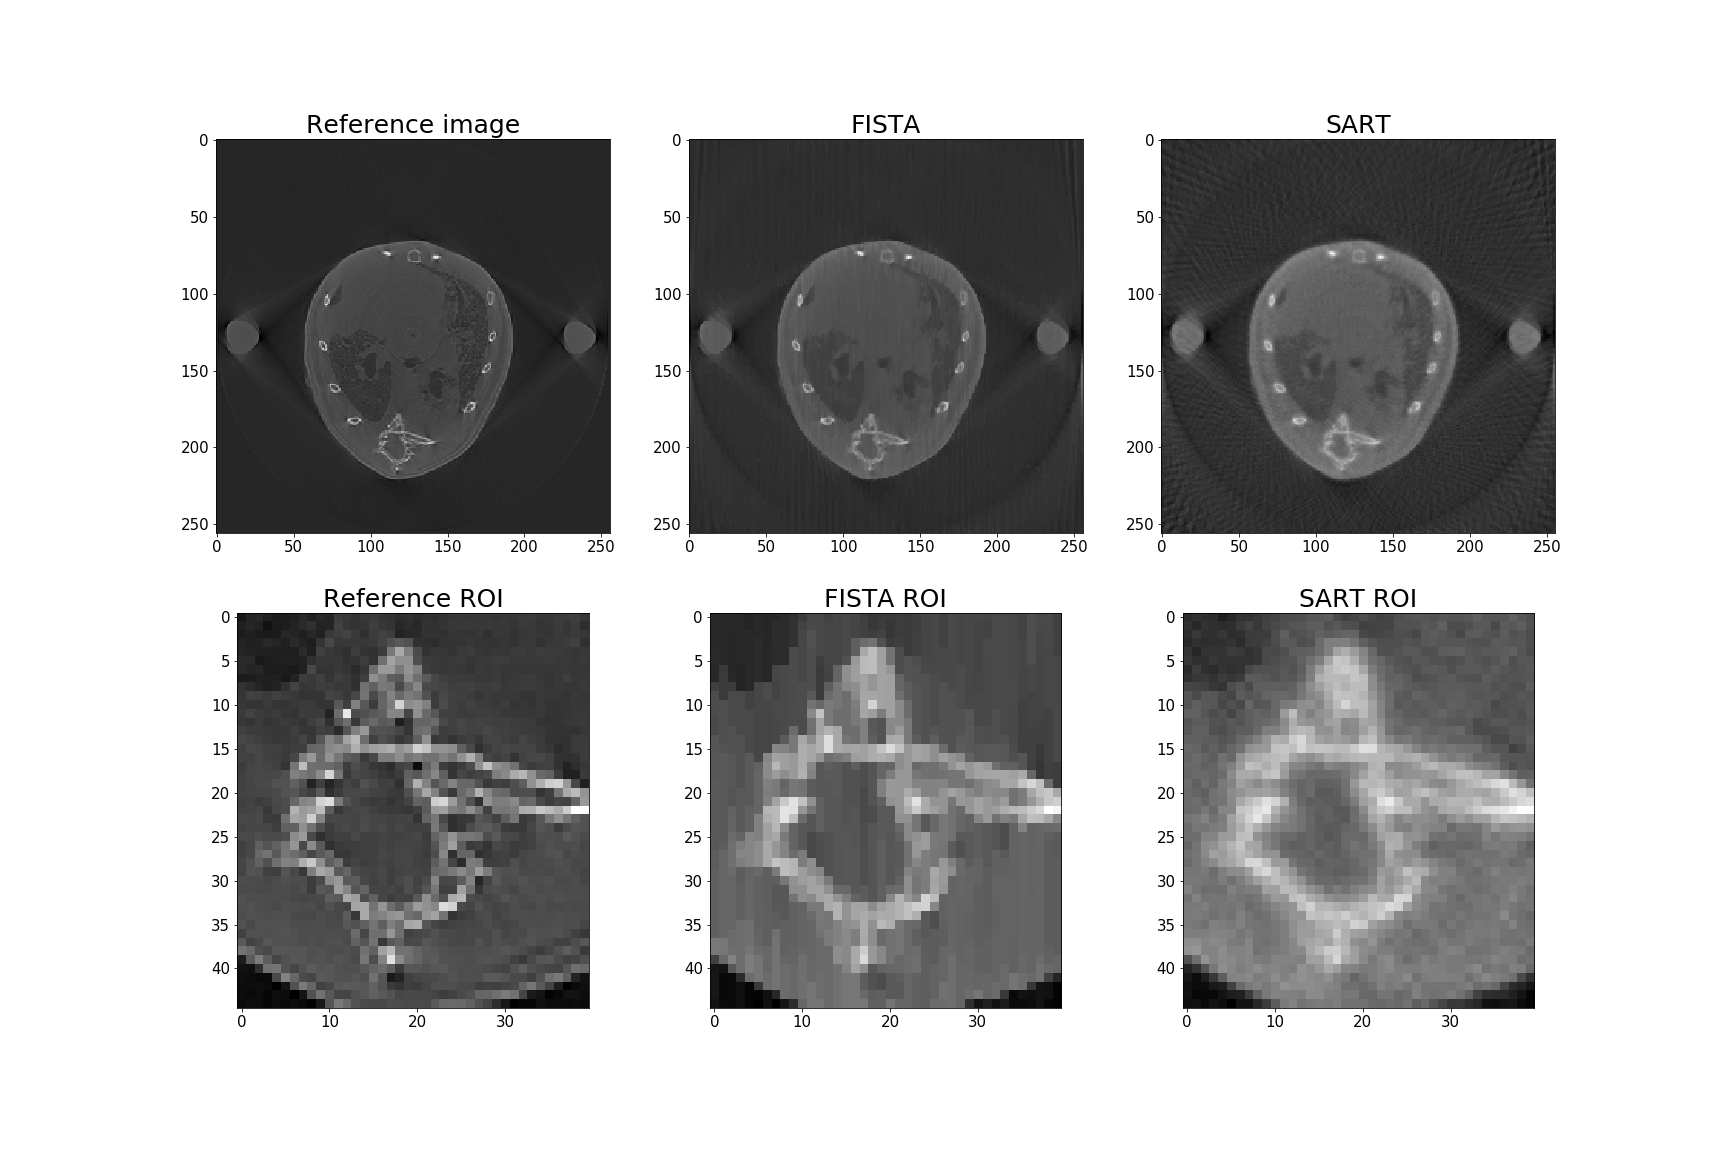
\includegraphics[height=0.35\paperheight]{results/comparison90.png}
	\caption{Reconstructed image using FISTA and SART from the 90 views.}
	\label{fig:comparison90}
\end{figure}

\section*{Discussion}
In general, FISTA outperforms SART at reconstructing the image. By comparing reconstructions on the three different sinograms, we see that the SSIM and MSE is more stable with FISTA (Tables~\ref{tab:ssim},~\ref{tab:mse}. Therefore, FISTA creates more robust reconstructions with less data. The FISTA reconstruction also has sharper edges compared to the SART reconstruction. This is especially apparently as fewer views are used (Figure~\ref{fig:comparison270}). The two methods also appear to handle noise differently. In the 90 view reconstruction, the SART reconstruction contains wavy patterns whereas the FISTA reconstruction contains vertical bands (Figure~\ref{fig:comparison90}). This may explain why the FISTA reconstruction is worse over the ROI because the ROI contains many horizonal and diagonal segments that are blurred by the vertical bands in the reconstruction.

\newpage
% Full image reconstructions
\setcounter{figure}{0}
\renewcommand{\thefigure}{S\arabic{figure}}
\begin{figure}[h]
	\centering
	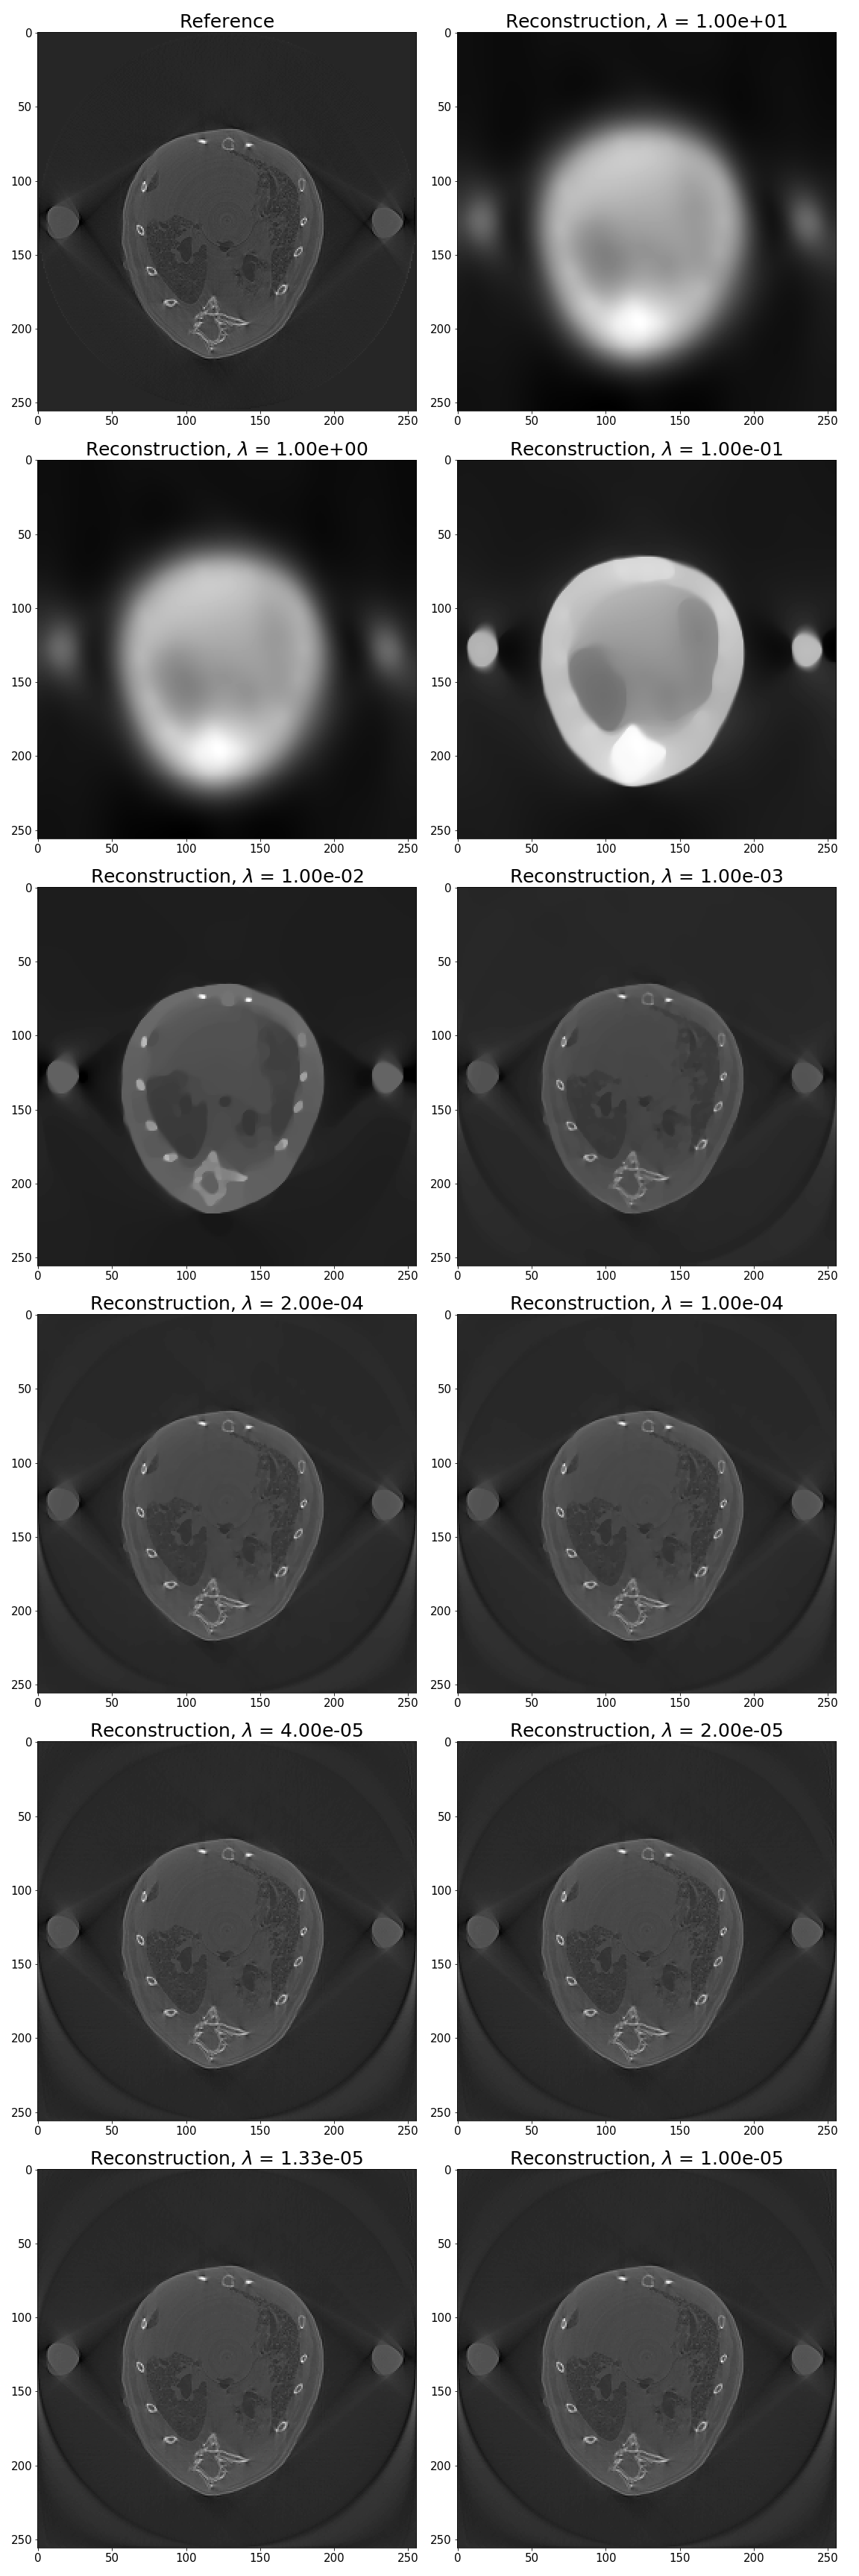
\includegraphics[height=0.8\paperheight]{results/fistaFullImages.png}
	\caption{FISTA reconstruction from full sinogram with different values of $\lambda$.}
	\label{fig:fullReconstructions}
\end{figure}

\end{document}
